
% ページフォーマットの指定
\documentclass[twocolumn]{jsarticle}

  % 外部パッケージの導入
  % 引用
  \usepackage{cite}
  % 画像の出力
  \usepackage[dvipdfmx]{graphicx}

  % コマンドの定義
  \newcommand{\fig}[1]{{図~\ref{fig:#1}}}
  \newcommand{\tab}[1]{{表~\ref{tab:#1}}}

  % 画像元のパスの追加
  \graphicspath{{figure/}}
  
  % 文書本体の記述
  \begin{document}
  \title{プログレスレポート}
  \date{\today}
  \author{森健一郎\\配布対象:安藤先生}
  
  \maketitle
  
  \section{研究目的}
  プロセッサ・チップ上には,ホット・スポットと呼ばれる単位面積あたりの電力が大きい場所が存在する.ホット・スポットは,そうでない場所と比べて温度上昇が激しいため,プロセッサの故障を引き起こす可能性が高い.~\cite{Weste2010,Monsieur2001,Khan2010,Black1969,Viswanath2000}従って,ホット・スポットを生成する回路の消費電力を低下させる必要がある.

  ホット・スポットを生成する回路の1つに,発行キュー(IQ:issue queue)がある.IQ のサイズはプロセッサの世代が進むごとに大きくなっており,より深刻なホット・スポットとなっている.従って,IQ の電力削減に対する要求は非常に大きい.
  
  IQ の中で最も電力を消費するのは,タグ比較の回路である.タグ比較は,発行幅分のディスティネーション・タグとすべてのソース・タグで行われるため,電力効率が非常に悪い.そこで本研究では,ディスティネーション・タグとソース・タグの下位ビットが等しい命令についてのみ比較器を動作させることにより,動作する比較器の数を減少させ電力を削減する方法を提案する.

  提案手法は,次のように実現する.IQ を複数のセグメントに分割し,第 n セグメントには,第 1 ソース・タグの下位ビットが n である命令のみをディスパッチする.そして,ウェイクアップのタグ比較の際には,ディスティネーション・タグの下位ビットが,自身に割り当てられた命令の第1ソース・タグの下位ビットと等しいセグメントのみ,比較器を動作させてタグ比較を行う.この方法により,第1ソース・タグについての比較器の動作回数を「1/セグメント数」に減少させることができる.

  提案手法における欠点として,セグメントが詰まることによる性能低下が挙げられる.あるセグメントに空きがない状態で,そのセグメントにディスパッチされる命令が現れた場合を考える.この場合,他のセグメントにディスパッチすることはできないため,該当のセグメントに空きが出るまでディスパッチを停止する必要があり,これは性能低下に繋がる.本研究では,この欠点に対する対応策を考え,性能低下が許容できる範囲内に収まるようにする必要がある.

  また,その他の欠点として,第2ソース・タグの比較器の動作回数は削減できないことなどが挙げられる.これらの欠点に対しても十分に検討し,提案手法における電力削減及び性能の変化について評価を行う.

  \section{経過}

  \subsection{前回の経過}
  \begin{itemize}
    \item プロセッサ構成の検討
    \item 提案手法におけるタグ比較回路の遅延軽減方法の検討
    \item 提案手法のネットリスト生成プログラムの作成
  \end{itemize}
  \subsection{今回の経過}
    \begin{itemize}
      \item Simple Scalar におけるディスパッチ命令数を修正し提案手法の再測定を行った
      \item HSPICE による提案手法の遅延測定を行った
    \end{itemize}
  \section{活動報告}
  \subsection{SimpleScalar の修正と提案手法の再評価}
  SimpleScalar において,1 サイクルでディスパッチできる命令数が $decode\_width \times fetch\_speed$ となっていたのを,$decode\_width$ と変更し,提案手法の再評価を行った.

  SimpleScalar では,デコード幅($decode\_width$)に $fetch\_speed$ という変数をかけた命令数だけ各サイクルにディスパッチが可能となっている.だが,この設定は提案手法によるディスパッチのストールが発生した際に,提案手法に対して有利に働くと思われる.つまり,ディスパッチのストール後,素早く発行キューに命令が供給されるため,提案手法の欠点が緩和されると考えられる.

  そこで今回は,この設定をやめ,ディスパッチ命令数は単に$decode\_width$とした場合の提案手法による性能低下を再評価した.

  \begin{table}[htb]
    \caption{プロセッサの基本構成}
    \footnotesize
    \center
      \begin{tabular}{l|l} \hline \hline
       Pipeline width & 8 instructions wide for each of \\
       & fetch, decode, issue, and commit \\
       Reorder buffer & 256 entries \\
       IQ & 128 entries \\
       Load/Store queue & 128 entries \\
       Physical registers & 256(int) + 256(fp) \\
       Branch prediction & 12-bit history 4K-entry PHT gshare \\
       & 2K-set 4-way BTB \\
       & 10-cycle misprediction penalty \\
       Function unit & 4 iALU, 2 iMULT, \\
       &  3 FPU, 2 LSU \\
       L1 D-cache & 32KB, 8-way, 64B line \\
        & 2-cycle hit latency \\
       L1 I-cache & 32KB, 8-way, 64B line \\
        &  2-cycle hit latency \\
       L2 cache & 2MB, 16-way, 64B line \\
        & 12-cycle hit latency \\  
       Main memory & 300-cycle latency \\
       & 8B/cycle bandwidth \\ 
       Prefetch & stream-based,32-stream tracked,  \\ 
       & 16-line distance, 2-line degree, \\
       & prefetch to L2 cache \\ \hline
    \end{tabular}
    \label{tab:base_config}
  \end{table}

\begin{table}[htb]
  \caption{提案手法のパラメータ構成}
  \footnotesize
  \center
    \begin{tabular}{l|l} \hline \hline
    切り替えインターバル & 10K instructions \\
    ISR しきい値 & 15\% \\
    LLC MPKI しきい値 & 2.0 \\ \hline 
  \end{tabular}
  \label{tab:segmentedIQ_config}
\end{table}

  \subsubsection{評価環境}
  \label{sec:config}
  評価環境について説明する.シミュレータには SimpleScalar をベースに修正を加えたものを使用した.表\ref{tab:base_config}にプロセッサ構成を示す.また,提案手法の SWITCH 方式に関するパラメータは\tab{segmentedIQ_config}に示す.
  
  測定ベンチマークには,SPEC CPU 2017 ベンチマークのうち,int 系 9 本と fp 系 9 本の計 18 本を使用した.ベンチマークの測定区間は,プログラムの先頭から 16G 命令をスキップした後の 100M 命令である.

  
  \begin{figure*}[ht]
    \centering
    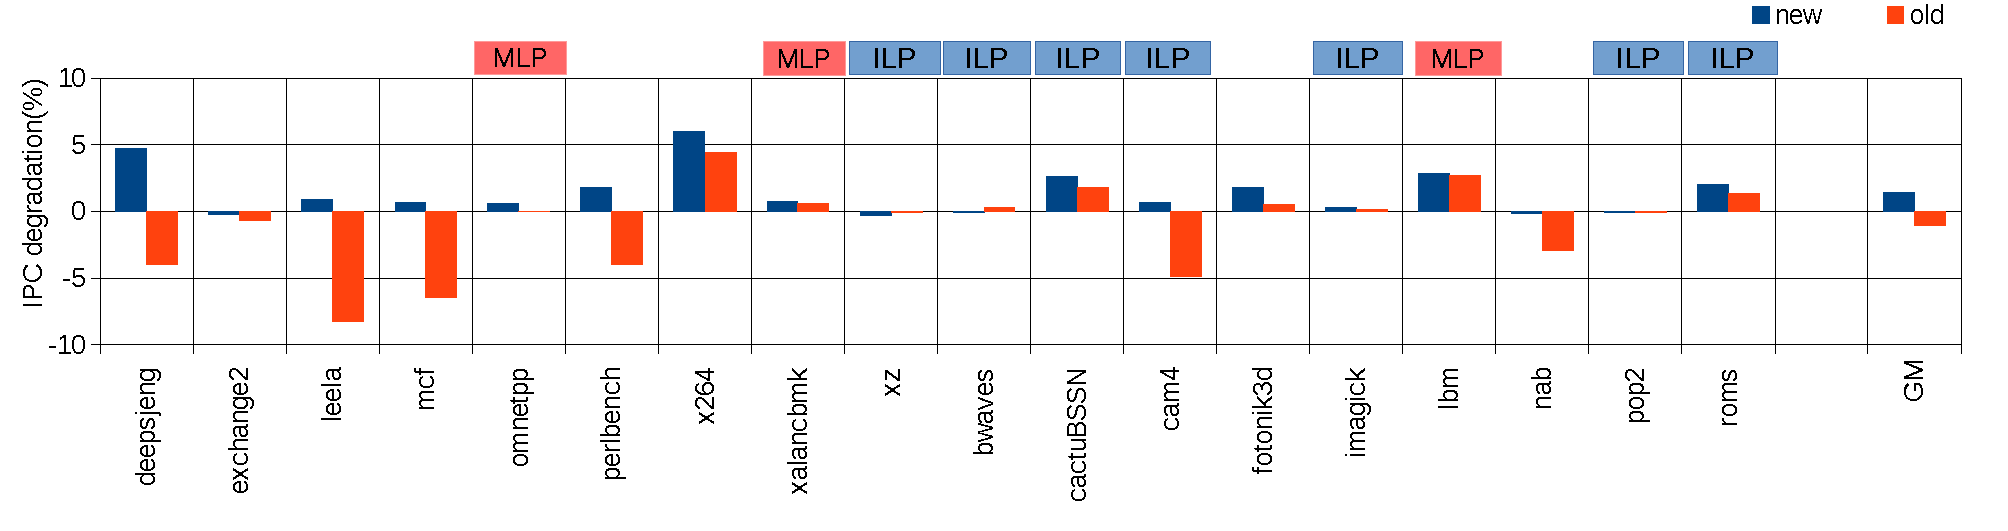
\includegraphics[width=0.99\hsize]{old_ipc.pdf}
    \caption{新実装と旧実装の比較(性能低下率)}  
    \label{fig:old_ipc}
  \end{figure*}

  \subsubsection{評価結果:旧実装との比較}
  ディスパッチ命令数の計算方法を変えた場合の提案手法による性能低下を\fig{old_ipc}に示す.当図は各ベンチマーク毎の提案手法による性能低下率を示している. old がディスパッチ命令数 $decode\_width \times fetch\_speed$ である旧実装を,new がディスパッチ命令数 $decode\_width$ である新実装の結果を表す.なお,セグメント数は旧実装で最適であったメイン・セグメント 16,サブ・セグメント 2 としている.

  図より,新実装は旧実装と比較して性能低下率が増加していることが分かる.特に,旧実装では性能が向上していたベンチマークにおいて,新実装では性能向上がおきていない.これは,ディスパッチがストールした際に,性能に与える影響が旧実装よりも新実装のほうが大きくなっているためと言える.

  \begin{figure*}[ht]
    \centering
    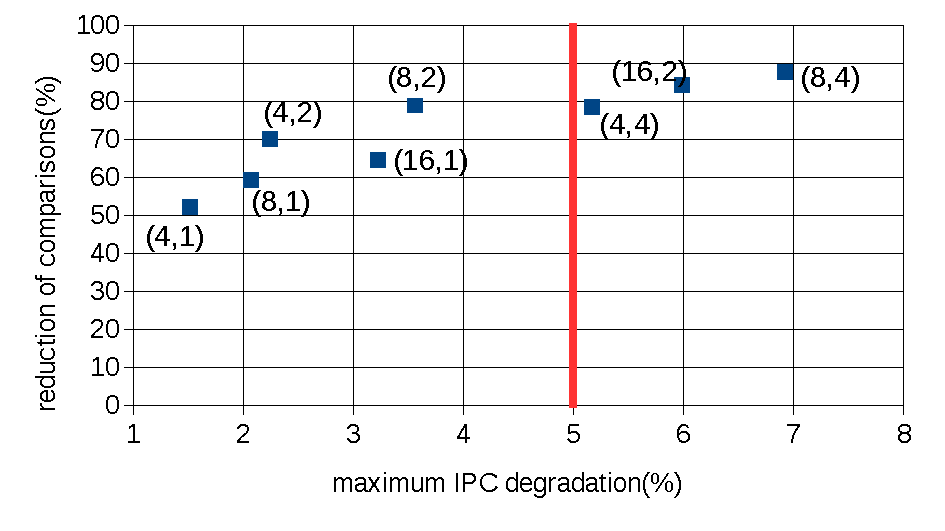
\includegraphics[width=0.99\hsize]{ipc_comp.pdf}
    \caption{新実装における提案手法の性能低下率とタグ比較回数削減率}  
    \label{fig:ipc_comp}
  \end{figure*}
  
  \begin{figure*}[ht]
    \centering
    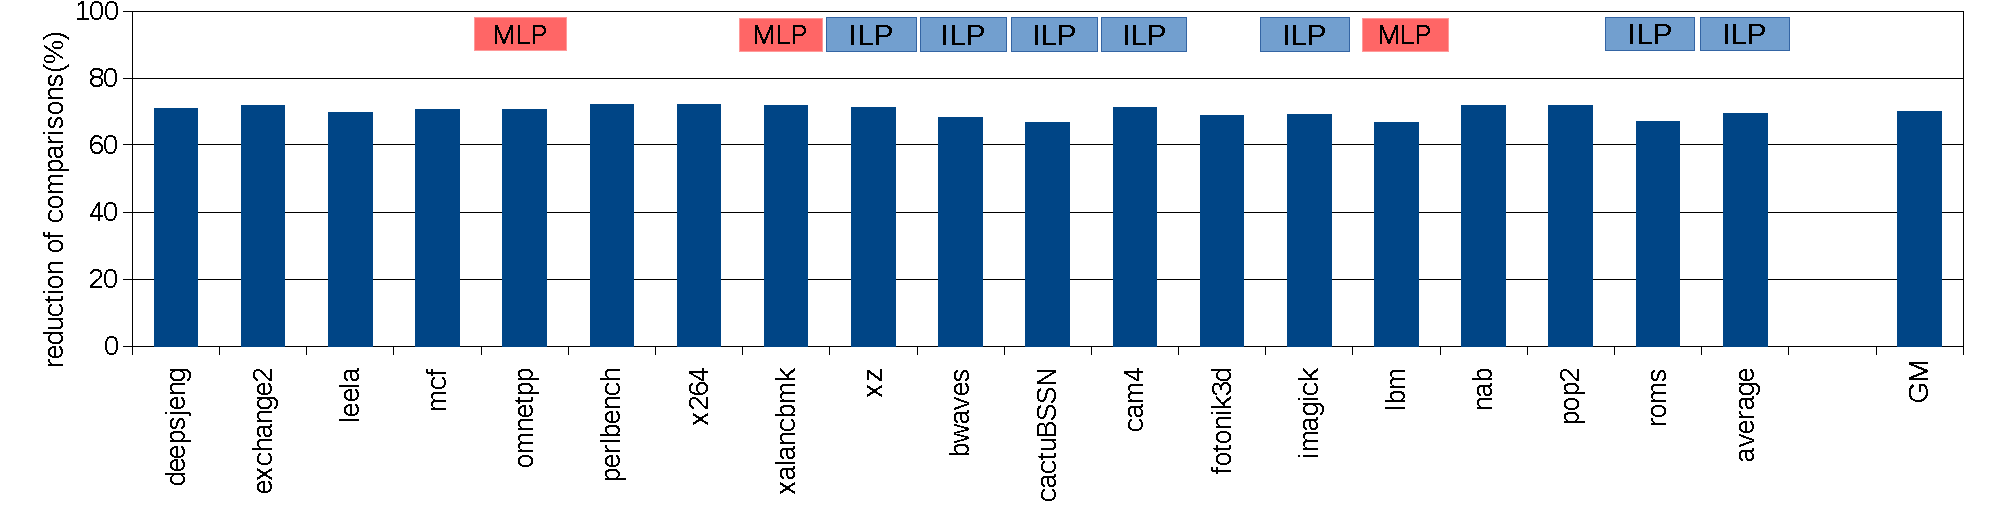
\includegraphics[width=0.99\hsize]{comp.pdf}
    \caption{提案手法によるタグ比較削減率(8, 2)}  
    \label{fig:comp}
  \end{figure*}

  \begin{figure*}[ht]
    \centering
    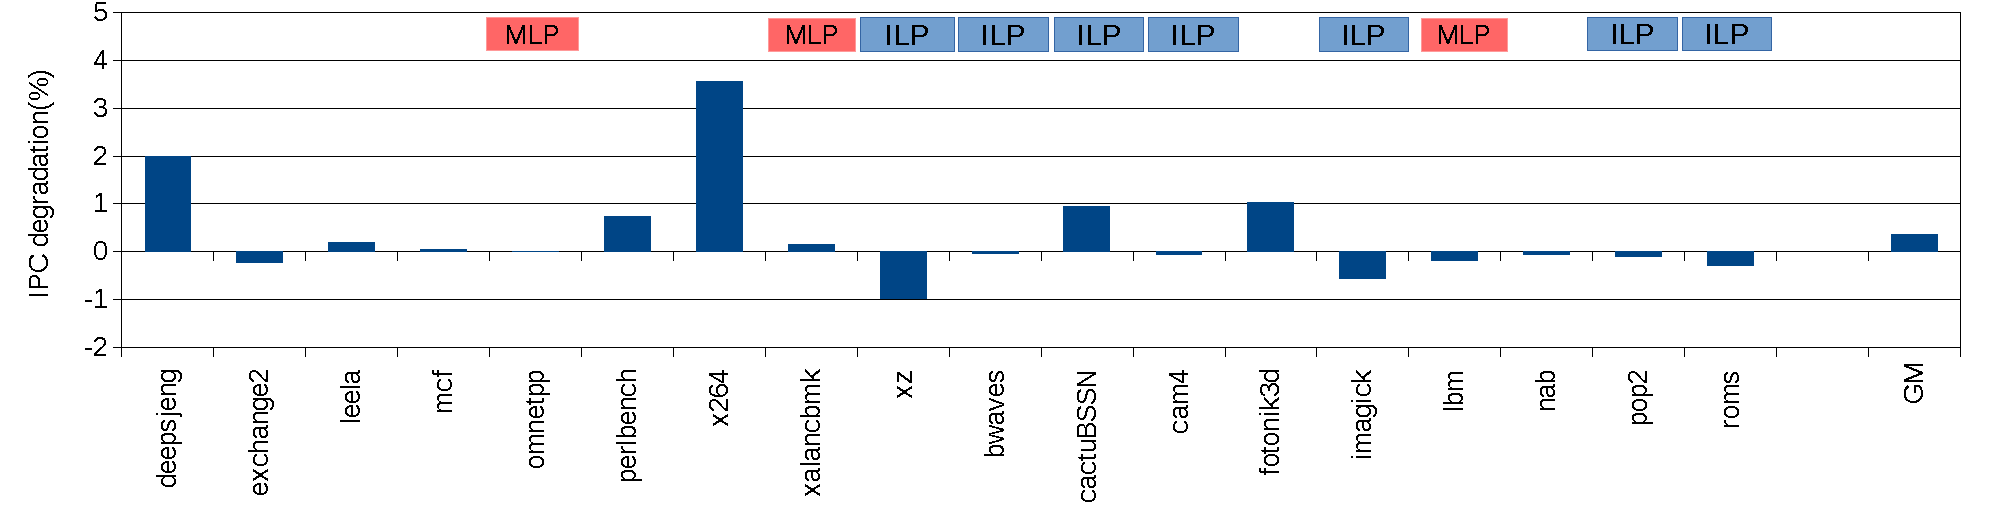
\includegraphics[width=0.99\hsize]{ipc.pdf}
    \caption{提案手法による性能低下率(8, 2)}  
    \label{fig:ipc}
  \end{figure*}
  \subsubsection{評価結果:新実装における提案手法のチューニング}
  新実装において,提案手法のチューニングを再度行った.チューニングする項目としては,メイン及びサブ・セグメント数である.以下の条件を満たすセグメント数の組み合わせを最適と評価する.なお,その他のパラメータ(SWITCH 方式で使用するしきい値など)は,旧実装の場合と同様としている.

  \begin{itemize}
    \item 性能低下が全ベンチマークで 5\% 以下である
    \item タグ比較回数の削減率が最も大きい
  \end{itemize}

  評価結果を\fig{ipc_comp}に示す.同図の横軸は,測定ベンチマークのうち最も性能低下が大きかったベンチマークにおける性能低下率を,縦軸はタグ比較回数削減率の平均を表している.また,図中に (メイン・セグメント数, サブ・セグメント数) の形式でセグメント数を示している.

  同図より,性能低下が 5\% (赤いライン)以下である組み合わせのうち,最もタグ比較回数が削減できているのは,(8, 2) である.従って新実装では,メイン・セグメント数が 8,サブ・セグメント数が 2 の場合が最適であると言える.

  (8, 2)の場合の各ベンチマーク毎のタグ比較回数削減率を\fig{comp}に,性能低下率を\fig{ipc}に示す.タグ比較回数削減率は平均で 78\%となっている.また,性能低下率の最大値は 3.5\%,平均は 0.3\% となっている.

  なお,旧実装でのタグ比較回数削減率は 85\% 程度であり,新実装では削減率が低下していることが分かる.これは,新実装は旧実装と比較して性能にシビアであり,セグメント数を大きく出来ないためである.
  \begin{figure*}[ht]
    \centering
    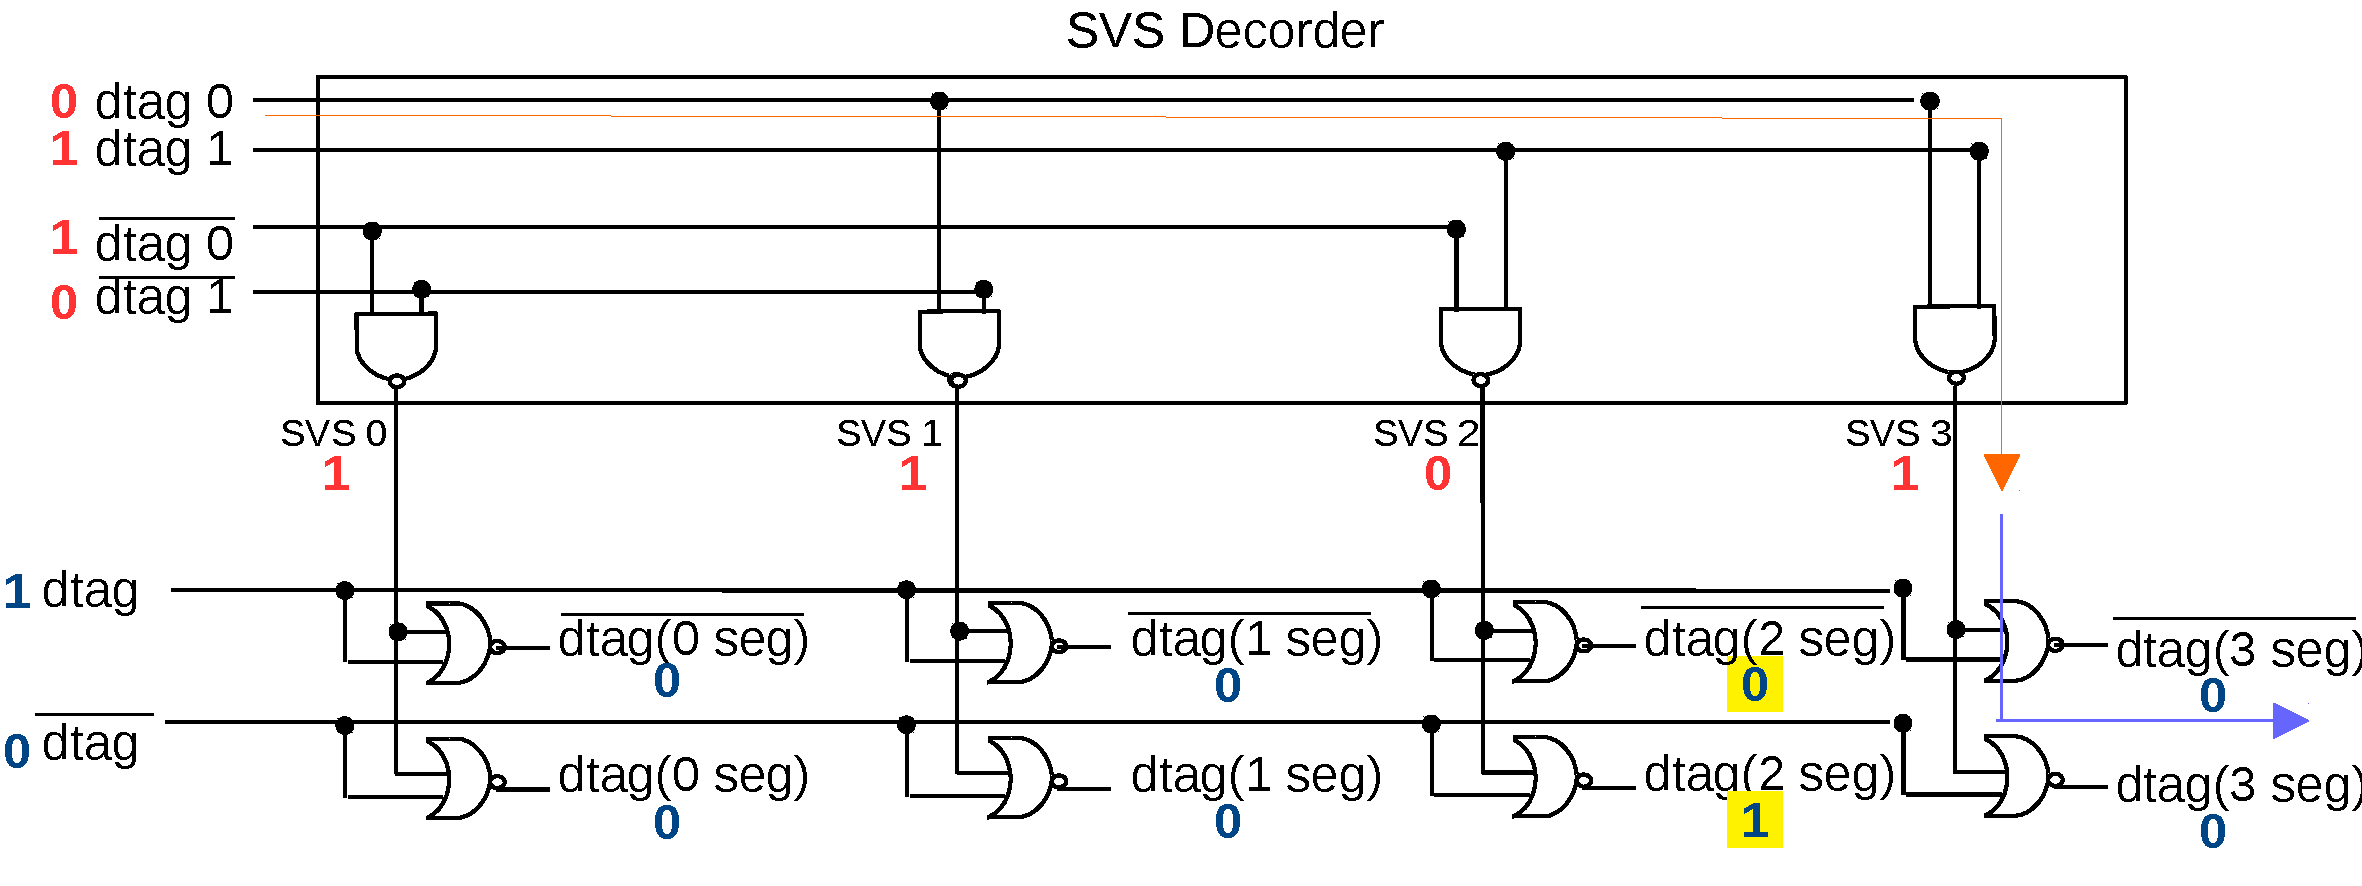
\includegraphics[width=0.99\hsize]{svs_decorder.pdf}
    \caption{SVS 回路}  
    \label{fig:svs_decorder}
  \end{figure*}

  \subsection{提案手法の遅延の評価}
  松田のネットリスト生成プログラムを修正し,提案手法におけるタグ比較回路の遅延測定を行った.しかし,おそらくネットリストに不具合があり,SVS の遅延時間が想定されるよりも大きすぎるという問題が発生している.

  \fig{svs_decorder}に,作成した回路のうち SVS に関連する部分を示す.SVS(Segment Valid Signal) は,各セグメントでの比較が有効であるかどうかを表す信号で,ディスティネーション・タグの下位ビットの NAND により生成される.図の例はセグメント数が 4 の場合であり,例えばタグの下位 2 ビットが $10_2$である場合には, SVS2 のみ 0 となり,他の SVS は全て 1 となる.

  SVS 信号はディスティネーション・タグのうち SVS に用いなかった高位ビットと NOR を取り,各セグメントの CAM に入力される.(ゲート数を削減するため,NOR を用い,かつタグの反転信号を入力している.つまり,\\$validated \ dtag = dtag \ AND \ SVS = dtag\_bar \ NOR \ SVS\_bar$)
  
  これによって,タグ比較が有効なセグメントでのみタグが入力され,そうでないセグメントではタグの正転信号と反転信号のどちらも 0 が入力され,CAM は電力を消費しない.

  \begin{table}[htb]
    \caption{ウェイクアップの遅延時間(ps)}
    \footnotesize
    \center
      \begin{tabular}{l|l} \hline \hline
       from tagRAM & 24.849 \\
       SVS & 36.192 \\
       broadcast & 105.72 \\ \hline
    \end{tabular}
    \label{tab:delay}
  \end{table}

  松田のネットリスト生成プログラムを修正して,SVS を含む提案手法のウェイクアップ回路の遅延測定を行った.表の各期間は次の意味を持つ.
  \begin{itemize}
    \item from tagRAM:tagRAM から SVS  の入力まで
    \item SVS:SVS 信号の生成(\fig{svs_decorder}における赤い矢印)
    \item broadcast:SVS により有効化したタグのブロードキャスト(図中の青い矢印) 
  \end{itemize}
  その結果,SVS 信号の遅延(\fig{svs_decorder}における赤い矢印)が想定していたよりも大幅に大きかった.具体的には\tab{delay}の通りである.SVS は今回の測定で 3 入力の NAND であるため,遅延はここまで大きくはならないはずであり,ネットリストに問題がある可能性が高い.現在,原因はわからずこの問題は解決していない.
  
  \section{研究計画}
  
  \begin{itemize}
    \item 修士論文を書く
  \end{itemize}
  
%  \section{関連文献}
  
  
  % 参考文献
  \bibliographystyle{../Config/andolab2} 
  \bibliography{../Config/ref}
  
  \end{document}
  